\scanpage{43}
Une application polynomiale homogène \inserted{de degré $n$} $\Phi:\underset{\sim}{M}\longrightarrow\underset{\sim}{N}$ définit par la formule
\[
\Phi\left(\sum_1^r t_ix_i\right)=\sum_{p_1+\cdots+p_r=n}\Phi_{p_1\cdots p_r}(x_1,\ldots,x_r)t_1^{p_1}\cdots t_r^{p_r}
\]
[les $t_i$ des indéterminées] des applications polynomiales
\[
\Phi_{p_1\cdots p_r}:\quad\unsure{\underset{\sim}{M}|\underline M}\times\cdots\times\underline M\unsure{\longrightarrow|\mathrel{\text{---}}}\underline N
\]
multihomogènes de degrés $p_1,\ldots,p_r$, d'où des applications
\[
\varphi_{p_1,\ldots,p_r}:\quad\underbrace{M\times\cdots\times M}_{r}\longrightarrow N
\]
(définies si $r\geq1$, $p_1,\ldots,p_r\geq0$, $\sum p_i=n$). Ces applications sont reliées par des relations
\[
\varphi_{p_1,\ldots,p_r}\deleted{\unsure{\varphi}}\left(\sum_{1\leq i\leq s_1}x_{1,i},\ \sum_{1\leq i\leq s_2}x_{2,i},\ \ldots\sum_{1\leq i\leq s_r}x_{r,i}\right)
=\sum_{\left\{\substack{\sum_{1\leq i_1\leq s_1}q_{1,i_1}=p_1\\\sum_{1\leq i_2\leq s_2}q_{\unsure{1|2},i_2}=p_2\\\cdots\\\sum_{1\leq i_r\leq s_r}q_{r,\unsure{s_r|i_r}}=p_r}\right.}
\varphi_{q_{1,i_1},\ldots,q_{r,s_r}}(x_{11},\ldots,\unsure{x_{r,s_r}}
\]
\margin{\figure{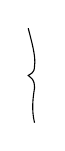
\begin{tikzpicture}[x=.4cm,y=.4cm]\draw (0,3) .. controls (.1,2.6) and (.25,2.1) .. (.2,1.8) .. controls (.2,1.55) and (.05,1.55) .. (0,1.5) .. controls (.1,1.4) and (.2,1.4) .. (.2,1.1) .. controls (.15,.8) and (.1,.4) .. (.2,0);\end{tikzpicture}}il suffit quand \uline{un} des \unsure{argts|arguments} est \unsure{remplacé} par une somme de \uline{deux} termes}
\uline{Plus relations de symétrie.}

On suppose que l'on a \unsure{une|aussi} réciproque $\ldots\ldots$
\mspage{42}
